\documentclass[ngerman,compress]{beamer}

\mode<presentation>
{
  \useoutertheme[footline=titleinstituteauthor]{c4}
  \useinnertheme{circles}
  \usecolortheme{c4}
  %\setbeamercovered{transparent}
  \setbeamercovered{highly dynamic}
}

\usepackage{babel}
\usepackage[utf8]{luainputenc}
\usepackage{fontspec}
\usepackage{listings}
\usepackage{color}

% Multimedia
%\usepackage{multimedia}

% sets the listings style
\definecolor{sh_comment}{rgb}{0.12, 0.38, 0.18 } %adjusted, in Eclipse: {0.25, 0.42, 0.30 } = #3F6A4D
\definecolor{sh_keyword}{rgb}{0.3, 0.3, 0.875}  % #5F1441
\definecolor{sh_string}{rgb}{0.875, 0.85, 0.11} % #101AF9

\lstset{basicstyle=\tiny\ttfamily,
	showspaces=false,
	showtabs=false, 
	showstringspaces=false, 
	columns=fullflexible, 
	stringstyle=\color{sh_string},
	keywordstyle=\color{sh_keyword}\bfseries,
	commentstyle=\color{sh_comment}\itshape
	}

\title[STM32 - u23 2012]
{\textbf{STM32}\\u23 2013}

\author[andy <andy@koeln.ccc.de>]
{andy, florob, gordin, ike, meise, tobix, zakx}

\institute[Chaos Computer Club Cologne]
{
Chaos Computer Club Cologne e.V.\\
http://koeln.ccc.de \\
}

\date{Cologne\\2013-10-21}

\pgfdeclareimage[height=1cm]{barcode}{./c4-logo}
\logo{\pgfuseimage{barcode}}


% Folgendes sollte gelC6scht werden, wenn man nicht am Anfang jedes
% Unterabschnitts die Gliederung nochmal sehen möchte.
%\AtBeginSection[]
%{
%  \begin{frame}<beamer>
%    \frametitle{Gliederung}
%    \tableofcontents[currentsection,currentsubsection]
%  \end{frame}
%}

% Falls Aufzählungen immer schrittweise gezeigt werden sollen, kann
% folgendes Kommando benutzt werden:
%\beamerdefaultoverlayspecification{<+->}


\begin{document}

\begin{frame}
  \titlepage
\end{frame}

\AtBeginSubsection

\begin{frame}
  \tableofcontents
  % Die Option [pausesections] könnte nützlich sein.
\end{frame}


\section{Einführung}

\subsection{Zeitplan}
\begin{frame}
	%\frametitle{Erfa-Kreise}
	\begin{itemize}
		\item Einführung
		\begin{itemize}
			\item 2013-10-19 11:00 --- C99 Einführung
		\end{itemize}
		\item Reguläre Termine
		\begin{itemize}
			\item 2013-10-21 19:30 --- STM32-Einführung (heute)
			\item 2013-10-28 19:30 --- Peripherie des STM32
			\item 2013-11-04 19:30 --- Kommunikation mit anderen Bausteinen
			\item 2013-11-11 19:30 --- Kommunikation mit anderen Bausteinen (2)
			\item 2013-11-18 19:30 --- Projektarbeit
			\item 2013-11-25 19:30 --- Projektarbeit
			\item 2013-11-28 19:30 --- OpenChaos
		\end{itemize}
	\end{itemize}
\end{frame}

\subsection{Hardware}

\begin{frame}
	\frametitle{STM32F4 Discovery}
		\begin{columns}
			\column{1.5in}
				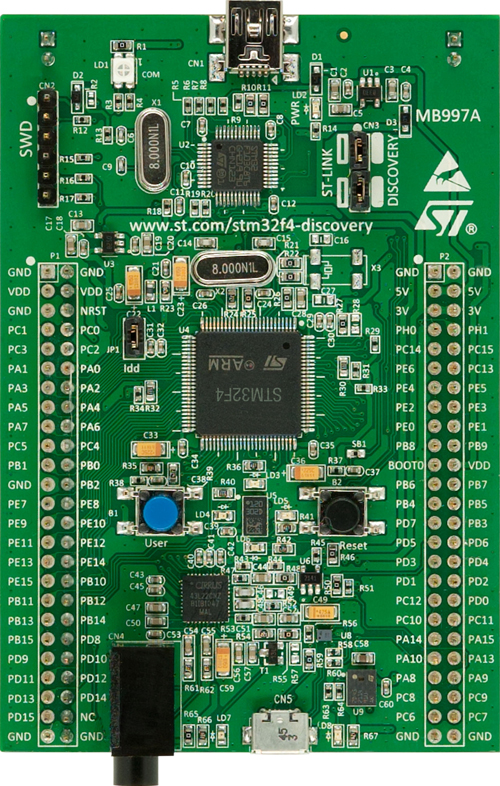
\includegraphics[height=2in]{stm32f4_discovery.jpg}
			\column{1.5in}
				\begin{itemize}
				\item STM32F407VGT6 32-bit ARM Cortex-M4F
				\item 1 MB Flash 
				\item 192 KB RAM (64KB CCM, 128KB SRAM)
				\item JTAG via ST-Linkv2
				\item USB OTG
				\item 100pin LQFP
				\end{itemize}
		\end{columns}
\end{frame}

\begin{frame}
	\frametitle{Boarddetails}
	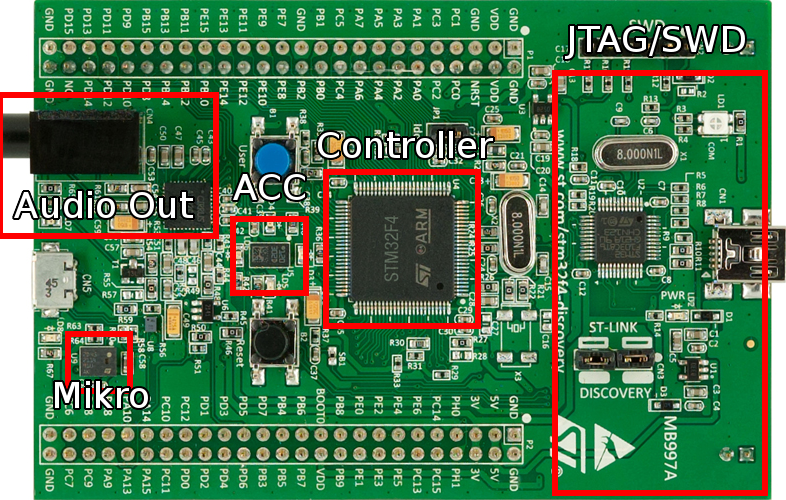
\includegraphics[height=2.5in]{stm32f4_discovery_beschriftet.png}
\end{frame}

\begin{frame}
	\frametitle{STM32F407}
	\begin{itemize}
		\item SoC = System on a Chip
		\item Lauffähiges Rechensystem komplett in einem Chip
		\item Nicht nur CPU + RAM, auch andere Peripherie:
		\begin{itemize}
			\item USARTs
			\item SPI-Controller
			\item I2C-Controller
			\item DCMI-(Kamera) Controller
			\item DMA-Engines
			\item GPIOs
			\item USB-Controller
			\item ... (siehe Datasheets später)
		\end{itemize}
		Bei nem "richtigen" PC ist oberer Kram alles im Chipsatz
	\end{itemize}
\end{frame}

\begin{frame}
	\frametitle{Chipübersicht}
	Datasheets sind eure Freunde! Ihr müsst allerdings auch erstmal lernen, wie man sie liest.
	\begin{itemize}
		\item Blockdiagramm: Datasheet STM32F407xx Seite 18
		\item Alternate Pin Functions: Datasheet STM32F407xx Seite 45
		\item Memory Map: Datasheet STM32F407xx Seite 63
	\end{itemize}
	Ist leider alles zu groß für die Slides :( \\
	Datasheets liegen im Libarary-Repo unter docs/
\end{frame}


\begin{frame}
	\frametitle{Externe Peripherie}
	Wir haben einiges an externen Bauteilen bestellt. China sollte irgendwann liefern.
	\begin{itemize}
		\item Servos
		\item Character- und (ein) Grafikdisplay
		\item Funkmodule
		\item Real-time clocks
		\item SD-Kartenadapter
		\item Magnetometer
		\item Ultraschall Entfernungssensoren
		\item 7-Segmentanzeigen
		\item Breadboards
		\item Kabel zum \$stuff zusammenstecken
		\item LEDs
		\item Buttons/Joysticks
	\end{itemize}
\end{frame}

\begin{frame}
	\frametitle{Projekte}
	Am Ende sollt ihr mit diesen Bausteinen was hübsches bauen. \\
	Erste Idee (vllt. etwas übertrieben): 3D-Scanner
	\begin{itemize}
		\item Zu scannendes Objekt sitzt auf einem Drehteller
		\item Ultraschall-Entfernungsmesser misst Entfernung zum Objekt
		\item Objekt wird etwas gedreht, nochmal gemessen
		\item Wenn eine Zeile fertig ist, Sensor in nächste Zeile schieben
		\item Irgendwann hat man dann vielleicht ein gescanntes 3D-Objekt
	\end{itemize}
	Sowas in der Art, gerne auch einfacher. Seid kreativ!
\end{frame}

\section{Software}

\subsection{Library}

\begin{frame}
	\frametitle{Unsere Library}
	\begin{itemize}
		\item Übernimmt Startup-Krempel und springt in main()
		\item Stell das Buildsystem zur Verfügung (Makefiles)
		\item Ihr könnt unseren Code benutzen, müsst aber nicht wenn ihr euch sicher seid, dass es ohne geht
		\item Zu finden unter \url{https://github.com/cccc/U23_2013_examples}
	\end{itemize}
\end{frame}

\begin{frame}
	\frametitle{Ordnerstruktur}
	\begin{columns}
			\column{3in}
	\begin{itemize}
		\item[apps/] Eure selbstgeschriebenen Apps
		\item[bare\_metal/] Beispiele ohne unsere lib
		\item[build/] Makefiles für das Buildsystem
		\item[docs/] Dokumentation, Datasheets, Schaltplan des Boards
		\item[tools/] Utilities (stlink-trace)
		\item[examples/] Beispielprogramme die unsere Library nutzen
		\item[libs/] Die Startup- und Peripherie-Libraries
	\end{itemize}
	\end{columns}
\end{frame}

\begin{frame}
	\frametitle{Neues Projekt anlegen}
	\begin{enumerate}
		\item Kopiert den Ordner \emph{hello\_word} in \emph{apps}
		\item Öffnet die Datei \emph{target.mak} in eurem \textbf{grade kopierten Ordner} und ändert die Variable \emph{TARGET} so, dass sie genau so heisst wie euer neuer Ordner
		\item Öffnet im Ordner \emph{apps} die Datei \emph{target.mak} und fügt zur Variable \emph{SUBDIRS} euren neuen (getrennt durch Leerzeichen) Ordnernamen hinzu
		\item Ihr könnt jetzt Sourcecode hinzufügen oder schreiben. Solltet ihr neue Dateien haben, die ihr kompilieren wollt, tragt sie in die Variable \emph{CCSOURCES} in der \emph{target.mak} ein.
	\end{enumerate}
\end{frame}

\begin{frame}
	\frametitle{Kompilieren und Flashen}
	\begin{itemize}
		\item Im Stammordner reicht ein \emph{make} um alles zu kompilieren
		\item \emph{make upload} lädt die Firmware 01\_blink auf euer Board
		\item Mit \emph{make upload-firmwarename} oder \emph{make upload FIRMWARE=firmwarename} ladet ihr eine bestimmte Firmware auf das Board
		\item In der Datei config.mk könnt ihr die Standardfirmware ändern
		\item Es gibt noch \emph{make upload-fast} was etwas schneller ist, was ihr benutzt spielt keine Rolle
	\end{itemize}
\end{frame}

\begin{frame} [fragile]
	\frametitle{Debuggen via gdb}
		\begin{lstlisting}
		$ ./debug.sh 
Connection to STM32 established. You can start debugging now
Ctrl+C or unplug USB to kill Connection 
		\end{lstlisting}
\end{frame}

\begin{frame} [fragile]
Auf anderer Shell:
	\begin{lstlisting}
$ arm-none-eabi-gdb u23_lib/examples/01_leds/obj/01_leds.elf 
GNU gdb (GNU Tools for ARM Embedded Processors) 7.4.1.20130312-cvs
[... license bla bla ...]
Reading symbols from /home/andy/Documents/CCC/U23_2013/examples/u23_lib/examples/01_leds/obj/01_leds.elf...done.

(gdb) target extended-remote :3333
Remote debugging using :3333
0x00000000 in ?? ()

(gdb) monitor reset init
target state: halted
target halted due to debug-request, current mode: Thread 
xPSR: 0x01000000 pc: 0x080004c4 msp: 0x10010000

(gdb) b main
Breakpoint 1 at 0x80001d4: file /home/andy/Documents/CCC/U23_2013/examples/u23_lib/examples/01_leds/src/main.c, line 8.

(gdb) c
Continuing.
Note: automatically using hardware breakpoints for read-only addresses.

Breakpoint 1, main () at /home/andy/Documents/CCC/U23_2013/examples/u23_lib/examples/01_leds/src/main.c:8
8		InitializeSystem();

(gdb) <weitere Befehle> 
[...]
	\end{lstlisting}
	Alternativ Eclipse. Gordin? Ach, sowas will doch niemand...
\end{frame}

\subsection{Codesamples}

\begin{frame}[fragile]
	\frametitle{Ein neues Programm}
	\begin{lstlisting} [language=C]
#include <System.h>
#include <stdio.h>

int main()
{
    // Do some basic initialization tasks
    InitializeSystem();

    // Initialize pins for LEDs
    InitializeLEDs();

    // Enable printf via trace macrocell (get output with 'make trace')
    EnableDebugOutput(DEBUG_ITM);

    //Turn on all LEDs
    SetLEDs(1 | 2 | 4 | 8);

    iprintf("Hello, World!\r\n");

    while(1);
}
	\end{lstlisting}
\end{frame}

\begin{frame}
	\frametitle{LEDs}
	\begin{itemize}
		\item LEDs kann man mit \emph{SetLEDs(int);} setzen
		\item Parameter ist eine Bitmaske
		\item LED 1 und 4 einschalten: (1<<0) | (1<<3)
	\end{itemize}
\end{frame}

\begin{frame}
	\frametitle{Accelerometer}
	\begin{itemize}
		\item Ein Accelerometer misst auf 3 Achsen (X, Y und Z) die Beschleunigung des Boards relativ zur Erde
		\item Zu gut Deutsch: Wie liegt das Board grade im dreidimensionalem Raum
		\item 3 Werte: Für jede Achse einen
	\end{itemize}
\end{frame}

\begin{frame} [fragile]
	\frametitle{Accelerometer Demo-Code}
	\begin{lstlisting} [language=C]
#include <System.h>
#include <Accelerometer.h>

int main()
{
    // Do some basic initialization tasks
    InitializeSystem();

    // Initialize pins for Accelerometer
    InitializeAccelerometer();

    // Calibrate the Accelerometer on the Start
    CalibrateAccelerometer();

    while (1)
    {
        int led = 0;
        int8_t Data[3] = {};

        // Read new Data
        ReadCalibratedAccelerometerData(Data);

        //... do some fancy WiiMote-Style shit ...
    }
}

	\end{lstlisting}
\end{frame}

\begin{frame}
	\frametitle{Debug Output per ITM}
	\begin{itemize}
		\item STM hat eine Trace-Makrozelle (ITM = Integrated Trace Macrocell)
		\item Einschalten per \emph{EnableDebugOutput(DEBUG\_ITM);}
		\item \emph{make trace} startet dann das trace utility
		\item Controller wird resettet und ihr seht alles, was ihr per \emph{printf()} ausgebt
	\end{itemize}
\end{frame}

\begin{frame}
	\frametitle{Debug Output per Serial}
	\begin{itemize}
		\item Debugging per Serial einschalten mit \emph{EnableDebugOutput(DEBUG\_USART);}
		\item Danach kann man \emph{printf()} benutzen
		\item Benutzt wird UART2 mit TX-Pin PA2 und RX-Pin PA3
	\end{itemize}
\end{frame}


\section{git}

\subsection{git}

\begin{frame}
	\frametitle{git}
	\begin{itemize}
		\item git ist ein Versionskontrollsystem
		\item Verwaltet alle Arten von Quellcode
		\item Lässt euch Änderungem, die ihr an Quellcode gemacht habt, verteilen
		\item Wir benutzen es für unsere Software
		\item Hier nur kurze Einführung
		\item Im Wiki stehen zwei längere Howtos:
		\item http://try.github.com/
		\item http://githowto.com/
	\end{itemize}
\end{frame}

\subsection{Befehle}

\begin{frame} [fragile]
	\frametitle{git clone <url>}
	\begin{itemize}
		\item Lädt das Repository vom Server und legt euch eine lokale Kopie an
	\end{itemize}

	\begin{lstlisting}
~ git clone git://github.com/cccc/U23-Library.git
Cloning into 'U23-Library'...
remote: Counting objects: 971, done.
remote: Compressing objects: 100% (713/713), done.
remote: Total 971 (delta 455), reused 739 (delta 223)
Receiving objects: 100% (971/971), 1.50 MiB | 650 KiB/s, done.
Resolving deltas: 100% (455/455), done.
	\end{lstlisting}
\end{frame}

\begin{frame} [fragile]
	\frametitle{git init}
	\begin{itemize}
		\item Erstellt euch ein neues lokales Repository
	\end{itemize}
	\begin{lstlisting}
~ git init
Initialized empty Git repository in /home/andy/Desktop/test/.git/
	\end{lstlisting}
\end{frame}

\begin{frame} [fragile]
	\frametitle{git status}
	\begin{itemize}
		\item Zeigt einem Dateistatus an
	\end{itemize}
	\begin{lstlisting}
~ git status
# On branch master
#
# Initial commit
#
# Untracked files:
#   (use "git add <file>..." to include in what will be committed)
#
#	testfile
nothing added to commit but untracked files present (use "git add" to track)
	\end{lstlisting}

\end{frame}

\begin{frame} [fragile]
	\frametitle{git add <filename>}
	\begin{itemize}
		\item Fügt eine Datei dem Index hinzu
		\item Damit weiß git, dass es diesen Inhalt der Datei beachten soll
		\item Muss für alle Dateien gemacht werden mit deren Inhalt man was gemacht hat
		\item Geht auch direkt auf ganzen Ordnern
	\end{itemize}
	\begin{lstlisting}
~ git add testfile
	\end{lstlisting}
\end{frame}

\begin{frame} [fragile]
	\frametitle{git commit}
	\begin{itemize}
		\item Fasst den aktuellen Index zusammen zu einem commit
		\item Commit = ein Änderungssatz zu einer bestimmten Sache
		\item Jeder Commit bekommt eine Commitmessage der ihn beschreibt, sodass andere Leute nachvollziehen können, was ihr gemacht habt
	\end{itemize}
	\begin{lstlisting}
~ git commit -m "Neues file hinzugefuegt"
[master (root-commit) d9ca032] Neues file hinzugefuegt
 0 files changed
 create mode 100644 testfile
	\end{lstlisting}
\end{frame}

\begin{frame} [fragile]
	\frametitle{git rm <filename>}
	\begin{itemize}
		\item Löscht eine Datei
	\end{itemize}
	\begin{lstlisting}
~ git rm testfile 
rm 'testfile'
	\end{lstlisting}
\end{frame}

\begin{frame} [fragile]
	\frametitle{git mv <source> <destination>}
	\begin{itemize}
		\item Verschiebt eine eine Datei
		\item Wird auch zum Umbenennen verwendet
	\end{itemize}
	\begin{lstlisting}
~ git mv testfile neuesfile
~ git status
# On branch master
# Changes to be committed:
#   (use "git reset HEAD <file>..." to unstage)
#
#	renamed:    testfile -> neuesfile
#
	\end{lstlisting}
\end{frame}

\begin{frame}
	\frametitle{Remotes}
	\begin{itemize}
		\item Remotes sind Zeiger auf andere Repositories des selben Projekts
		\item Ihr könnt dahin pushen (falls ihr dir Rechte habt) oder davon pullen
		\item Der C4 hat ein Repo, ihr habt alle Repos
		\item Ihr pusht also immer nur in euer eigenes Repo und pullt von allen anderen in eurem Team oder vom C4 um ihre neuen Änderungen zu bekommen
		\item Remote hinzufügen geht so: \emph{git remote add <remotename> <remoteurl>}
	\end{itemize}
\end{frame}

\begin{frame}
	\frametitle{git push}
	\begin{itemize}
		\item Schiebt eigene Änderungen auf den Server
		\item Server ist nicht zwingend notwendig, aber praktisch um Änderungen zu verteilen
		\item Wenn jemand anders in der Zwischenzeit Änderungen gepusht hat, die ihr noch nicht habt, kann es sein, dass es abgelehnt wird -- dann einmal pullen (ggf. mergen) und wieder pushen
		\item Beispiel: \emph{git push [remote [branchname]]}
	\end{itemize}
\end{frame}

\begin{frame}
	\frametitle{git pull}
	\begin{itemize}
		\item Holt Änderungen vom Server
		\item Beispiel: \emph{git push [remote [branchname]]}
	\end{itemize}
\end{frame}

\begin{frame}
	\frametitle{git log}
	\begin{itemize}
		\item Zeigt euch alle Commits der Reihe nach an
		\item gitk ist das selbe in grafisch
	\end{itemize}
\end{frame}

\section{Aufgaben}
\subsection{Aufgaben}
\begin{frame}
	\frametitle{Aufgaben}
	\begin{enumerate}
		\item Falls ihr noch kein Board habt, geht zum Andy und holt euch eins
		\item Legt euch nen github Account an
		\item Forkt das U23 Projekt des C4s (C4-Account: cccc)
		\item Clonet euren neuen Fork
		\item Fügt das C4-Repo als upstream remote hinzu (\emph{git remote add upstream \url{https://github.com/cccc/U23_2013_examples.git}})
		\item Legt ein neues Projekt an
		\item Lasst LEDs blinken
		\item Gebt euch mal Debugging output aus (per ITM)
		\item Vielleicht schafft ihr es schon Accelerometerwerte per Debugoutput auszugeben
		\item Probiert mal mit dem GDB zu Debuggen
	\end{enumerate}
\end{frame}

\end{document}
